%%%%%%%%%%%%%%%%%%%%%%%%%%%%%%%%%%%%%%%%%
% University/School Laboratory Report
% LaTeX Template
% Version 3.1 (25/3/14)
%
% This template has been downloaded from:
% http://www.LaTeXTemplates.com
%
% Original author:
% Linux and Unix Users Group at Virginia Tech Wiki 
% (https://vtluug.org/wiki/Example_LaTeX_chem_lab_report)
%
% License:
% CC BY-NC-SA 3.0 (http://creativecommons.org/licenses/by-nc-sa/3.0/)
%
%%%%%%%%%%%%%%%%%%%%%%%%%%%%%%%%%%%%%%%%%
% Technical Report on Parallax Correction of Tobii Glasses Eye Tracker.
%
% Author:
% Jin-Hwa Kim (jhkim@bi.snu.ac.kr)        07/10/2014
%
%%%%%%%%%%%%%%%%%%%%%%%%%%%%%%%%%%%%%%%%%
%----------------------------------------------------------------------------------------
% PACKAGES AND DOCUMENT CONFIGURATIONS
%----------------------------------------------------------------------------------------

\documentclass{article}

\usepackage{graphicx} % Required for the inclusion of images
\usepackage{natbib} % Required to change bibliography style to APA
\usepackage{url}
\usepackage{gensymb}

\setlength\parindent{0pt} % Removes all indentation from paragraphs

\renewcommand{\labelenumi}{\alph{enumi}.} % Make numbering in the enumerate environment by letter rather than number (e.g. section 6)

%\usepackage{times} % Uncomment to use the Times New Roman font

%----------------------------------------------------------------------------------------
% DOCUMENT INFORMATION
%----------------------------------------------------------------------------------------

\title{Technical Report on Parallax Correction \\
of Tobii Glasses Eye Tracker} % Title

\author{Jin-Hwa \textsc{Kim}} % Author name

\date{\today} % Date for the report

\begin{document}

\maketitle % Insert the title, author and date

\begin{center}
\begin{tabular}{l r}
Date Performed: & June 24, 2014 \\ % Date the experiment was performed
Partners: & Eun-Sol Kim \\ % Partner names
& Kyoung-Woon On \\
Instructor: & Professor Byoung-Tak Zhang % Instructor/supervisor
\end{tabular}
\end{center}

% If you wish to include an abstract, uncomment the lines below
% \begin{abstract}
% Abstract text
% \end{abstract}

%----------------------------------------------------------------------------------------
% SECTION 1
%----------------------------------------------------------------------------------------

\section{Objective}

To determine that the effectiveness of the parallax correction as the post calibration procedure. 

% If you have more than one objective, uncomment the below:
%\begin{description}
%\item[First Objective] \hfill \\
%Objective 1 text
%\item[Second Objective] \hfill \\
%Objective 2 text
%\end{description}

\subsection{Definitions}
\label{definitions}
\begin{description}

\item[Calibration]
The calibration procedure manually moved the calibration point for the acquirement of the accurate gaze points. This internal calibration point is only valid while the glasses are not removed from the participant's head. Accuracy depends on the variety factors, which are right distance, exact points and light conditions, during the calibration procedure.

\item[Recalibration]
Tobii Glasses eye tracker, which is used by our experiment, provides the post calibration which can be conducted the calibration procedure after the eye movement recording. This is called as \textit{Post calibration} or \textit{recalibration}. In this technical report, we particularly describe the \textit{Post calibration} or \textit{recalibration} as the procedure for the parallax correction.

\item[Gaze Point]
Gaze point means literally the location that the participant gazes.

\item[Fixation Point]
Fixation point means the location that the participant fixes his or her gaze point for some time. Because the gaze points are always changing subtly even in the voluntary fixation state, the definition of the fixation is defined by the fixation filtering method. We used the system default fixation filter, I-VT fixation filter \citep{Salvucci2000}.

\item[Parallax Correction]
The displacement of the locations of the eye and the camera of the eye tracker induces the error of the measured gaze point. The changes in the distance to the target make the parallax, the more closer the target is causes the larger error. For details, refer to the \textit{Tobii Glasses User Manual} \citep{tobii_manual}.

\end{description} 
 
%----------------------------------------------------------------------------------------
% SECTION 2
%----------------------------------------------------------------------------------------

\section{Experiments}

To verify the improvement of the measurement of gaze points after the parallax correction, we used the Gaze Accuracy Test (GAT) in advance of the watching the video. The gaze accuracy test will show us how much accurate before and after the recalibration.

\subsection{Gaze Accuracy Test}
For the measurement of the accuracy of the gaze point, we prepared the test video which has the moving dot on the lattice background. Participants are instructed to patiently fixate on the dot while it is stationary. You can check the video on YouTube at \citet{GAT}.

\subsection{Method}
Before the recording of the participant's eye movements, we took the snapshot from the eye tracker. This snapshot (actually, the set of internal files) contains the information of the IR makers' location and its identities via the function of the device. For this, we can obtain coordinates of gaze points on the snapshot image. After applying the affine transformation featured by the snapshot, we get the media coordinates, which represents the positions on the video screen. The coordinates on the snapshot image $\mathbf{x}$ is transformed to the coordinates on the video screen $\mathbf{x^\ast}$ via the affine transformation matrix $\mathbf{A}$ is defined as the algebraic equation, 

\begin{center}
$\mathbf{x^\ast} = \mathbf{Ax},$\\
\end{center}

and the affine transformation matrix $\mathbf{A}$ is defined by the salient positions $\mathbf{X}$, for example, the positions of four corners, and its corresponding coordinates on the video screen $\mathbf{y}$ as

\begin{center}
$\mathbf{A} = \mathbf{yX'}pinv(\mathbf{XX'})$.
\end{center}


%----------------------------------------------------------------------------------------
% SECTION 3
%----------------------------------------------------------------------------------------

\section{Results and Conclusions}

We recorded eye movements during 45 seconds for the Gaze Accuracy Test. All five locations, four corners of a quarter sized square centered in the screen and the center point, are visited three times each, and each visit holds three seconds to fixate on it. Through this, we got 1158 fixation points in the test. Figure~\ref{fig:parallax-correction} shows the parallax correction (blue circle) improves the accuracy in comparison with the not applied one (red cross).

\begin{figure}
  \centerline{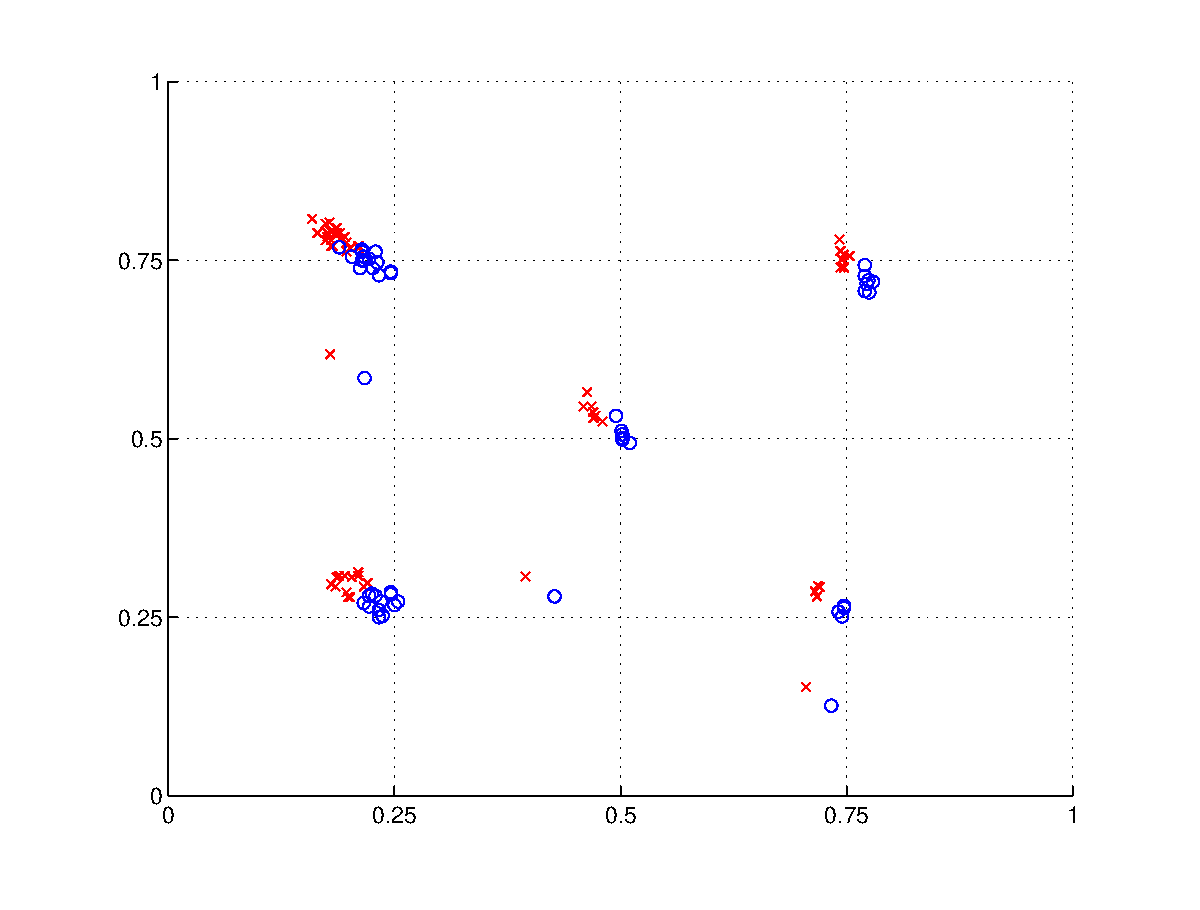
\includegraphics[width=86mm,trim=10mm 10mm 10mm 10mm]{./eps/parallax_correction.eps}}
  \caption{\textit{Parallax Correction} improves overall accuracy. We recorded 45 seconds of eye movements on the Gaze Accuracy Test. All five locations are visited three times, and each visit holds three seconds to fixate on it. Through this, we got 1158 fixation points in the test. Red crosses mean the fixation points without the parallax correction, which are recorded at 170 cm in front of the screen. Blue circles are with the parallax correction.}
  \label{fig:parallax-correction}
\end{figure}


%----------------------------------------------------------------------------------------
% SECTION 4
%----------------------------------------------------------------------------------------

\section{Discussion of Other Possible Solutions}

The parallax correction affects on the x-axis bias of the locations of eye movements. Because the displacement of the locations of the eye and the camera of the eye tracker induces the error of the measured gaze point (the camera of the eye tracker is placed in the right of the glass, horizontally.), for the changes in the distance to the target make the parallax. Therefore, the measurement error after the parallax correction may attribute to the calibration error. For the very accurate measurement of eye movements we have to conduct the verification procedure, however, considering of the range of foveal or central vision is around 2-5$^{\circ}$ (baseline) \citep{mcmorris2014acquisition}, it means that the perfect calibrated measurement may produce 2-5$^{\circ}$ error in the free-viewing task, this procedure can be a burden.

\cite{tatler2007central} shows the central fixation bias in the scene viewing task. According to Tatler's work, the possible explanations are three, which are expectancy, efficiency, and habitual re-centering. It makes the assumption of that the median of fixation positions is the center of the screen is plausible. Though we do not include the results in this report, the median-to-center adjustment dramatically corrects the poor calibrated measurements for watching video task, though it is not perfect with 6-7$^{\circ}$ error. We assume that the non-symmetric distribution of salient features in a video sequence raises the additional error to the baseline. Partly, the high-level interpretation of the given features also contributes to this influence \citep{tatler2005visual}.


%----------------------------------------------------------------------------------------
% BIBLIOGRAPHY
%----------------------------------------------------------------------------------------

\bibliographystyle{apalike}

\bibliography{kim2014parallax}

%----------------------------------------------------------------------------------------


\end{document}